\documentclass[conference]{IEEEtran}
\IEEEoverridecommandlockouts
\usepackage{cite}
\usepackage{amsmath,amssymb,amsfonts}
\usepackage{algorithm}
\usepackage{algpseudocode}
\usepackage{graphicx}
\usepackage{textcomp}
\usepackage{xcolor}
\usepackage{booktabs}
\usepackage{tikz}
\usetikzlibrary{arrows.meta,positioning}
\usepackage{enumitem}
\def\BibTeX{{\rm B\kern-.05em{\sc i\kern-.025em b}\kern-.08em
    T\kern-.1667em\lower.7ex\hbox{E}\kern-.125emX}}

\begin{document}

\title{CASCE: A Context-Aware Semantic Correlation Engine for eBPF-Based Cross-Layer PostgreSQL Security}

\author{
\IEEEauthorblockN{Jobin A J}
\IEEEauthorblockA{\textit{Dept. of Computer Science and Engineering} \\
\textit{TKM College of Engineering}\\
Kollam, India \\
}
\and
\IEEEauthorblockN{Asiya Salam}
\IEEEauthorblockA{\textit{Dept. of Computer Science and Engineering} \\
\textit{TKM College of Engineering}\\
Kollam, India}
\and
\IEEEauthorblockN{Adithyan M C}
\IEEEauthorblockA{\textit{Dept. of Computer Science and Engineering} \\
\textit{TKM College of Engineering}\\
Kollam, India}
\and
\IEEEauthorblockN{Sreedeep Rajeevan}
\IEEEauthorblockA{\textit{Dept. of Computer Science and Engineering} \\
\textit{TKM College of Engineering}\\
Kollam, India}
}

\maketitle

\begin{abstract}
PostgreSQL-level security mechanisms and Linux kernel-level instrumentation operate as two blind halves: PostgreSQL provides rich SQL and database-semantic context but has limited visibility into operating-system activity, while eBPF-based kernel monitoring observes process, file, and network activity without understanding SQL-level semantics. This paper presents CASCE, a Context-Aware Semantic Correlation Engine for PostgreSQL security, which bridges these layers by anchoring cross-layer correlation on process identity rather than heuristic timestamp or log-content matching. CASCE exploits PostgreSQL's process architecture, in which the postmaster creates a dedicated backend process for each client session, allowing database-session activity and operating-system activity associated with the same backend process to be correlated through process identity. The system instruments PostgreSQL executor activity directly through PostgreSQL Executor Hooks rather than relying exclusively on self-reported database logs, reducing dependence on conventional database logging and maintaining observability under database-log tampering. CASCE is organized into four algorithms, each with a distinct responsibility: Session-Anchored Correlation (SAC) attributes PostgreSQL and kernel events to their originating database sessions using process identity and process start time as the session key, tracing operating-system events through the process tree to a bounded depth when necessary; Incremental Cross-Layer Graph Construction builds a per-session heterogeneous factual graph from these attributed events without performing abstraction or threat judgment; Behavior Abstraction identifies higher-level behavioral patterns through structural, semantic, and temporal similarity against a curated behavior-template library, producing an enriched graph annotated with confidence scores while deliberately withholding threat labels; and Hybrid Cross-Layer Threat Detection combines a fast rule-based path with a Graph Attention Network scorer to produce a final session-level risk assessment and trigger alerts or, where warranted, automated response. By isolating threat judgment to the final stage, CASCE separates event attribution, behavioral interpretation, and threat classification, enabling independent validation of each processing stage. CASCE is being evaluated in a controlled PostgreSQL security environment containing PostgreSQL-semantic and cross-layer attack scenarios, including SQL-injection-to-role-escalation, database-driven operating-system activity, and insider-misuse scenarios, with evaluation covering individual attack detection, multi-stage attack-chain reconstruction, detection latency, precision, recall, and end-to-end processing overhead.
\end{abstract}

\begin{IEEEkeywords}
PostgreSQL security, PostgreSQL Executor Hooks, Linux kernel security, eBPF, cross-layer correlation, provenance graphs, intrusion detection, SQL query anomaly detection.
\end{IEEEkeywords}

\section{Introduction}

Modern relational database systems such as PostgreSQL sit at the center of almost every critical enterprise application, yet their built-in security mechanisms operate almost entirely in isolation within the database process itself. Extensions such as \texttt{pgAudit} record what a session executed at the SQL level, but cannot observe how that session came to exist -- whether it was opened by a legitimate application, a compromised credential, or a shell spawned through kernel-level privilege escalation. Conversely, Linux kernel security monitors built on eBPF observe system calls at low overhead, but lack domain context regarding what a \texttt{SELECT}, a \texttt{COPY FROM PROGRAM}, or a role grant signifies to the database running atop the kernel.

This visibility split is directly exploitable by Advanced Persistent Threats (APTs). An attacker who compromises a shell account, escalates privileges at the operating-system level, and subsequently executes malicious SQL statements produces an event chain that appears benign when either layer is analyzed independently. A kernel-only monitor sees an ordinary process spawning child processes; a database-only monitor sees a syntactically valid, authorized query. Only a system that correlates the kernel event stream and the database AST event stream as evidence of a single underlying session can reconstruct the complete attack story.

This paper presents \textbf{CASCE} (Cross-layer Session-Centric Environment for PostgreSQL Threat Detection), a cross-layer security framework that dynamically fuses eBPF kernel instrumentation with PostgreSQL Abstract Syntax Tree (AST) query executor events. CASCE anchors correlation on \emph{process identity} (backend PID ancestry up to depth $D_{\text{max}}=8$) rather than heuristic timestamp proximity: because PostgreSQL forks a backend process per client session, kernel-visible processes and database-visible sessions are structurally identical entities observed from dual instrumentation points.

The core contributions of this paper are:
\begin{enumerate}[leftmargin=*,itemsep=1pt,topsep=2pt]
\item \textbf{A Four-Stage Detection Architecture}: A modular pipeline comprising Session-Anchored Correlation (SAC), Heterogeneous Base Graph Construction, MITRE ATT\&CK Behavioral Abstraction ($S_{\text{struct}}, S_{\text{sem}}, S_{\text{temp}}$), and a Heterogeneous Graph Attention Network (\textbf{HeteroGATv2}) with hybrid risk scoring $R(S_i) = \alpha S_{\text{rule}} + (1-\alpha) S_{\text{GAT}}$.

\item \textbf{Declarative Counterfactual Dataset Engine}: A spec-driven synthetic generation framework (\texttt{datagen}) that enforces a cross-layer scope invariant (preventing OS activity presence from acting as a trivial shortcut label) and matched-pair counterfactual controls across fixed and varied execution dimensions.

\item \textbf{Multi-Domain Benchmark \& Rigorous Gating}: Evaluation across a 10,002-graph multi-domain corpus (Banking, E-Commerce, Healthcare, Logistics) using family-disjoint train/val/test splits and hard gating against 7 statistical shortcut baselines (node presence, bag-of-primitives, SQL-only, OS-only, graph size, rule-engine-alone, behavior-masked GAT), achieving \textbf{95.11\% Accuracy}, \textbf{95.46\% Recall}, and a \textbf{94.86\% F1-Score}.
\end{enumerate}

The remainder of this paper is organized as follows. Section~II surveys related work across database security, provenance tracking, and GNN intrusion detection. Section~III presents the CASCE system architecture and its four constituent algorithms. Section~IV details the spec-driven dataset generation, shortcut-gating protocol, and experimental setup. Section~V outlines the experimental setup, while Section~VI evaluates CASCE across multi-domain benchmarks and baseline models. Finally, Section~VII provides a discussion and Section~VIII concludes with directions for future work.

\section{Related Work}

Research relevant to CASCE spans five closely related areas: Linux kernel security and monitoring, provenance-based intrusion detection (PIDS), database security and database intrusion detection, cross-layer correlation, and AI-based log and graph anomaly detection. These research communities provide complementary capabilities, but differ in the level of system context they represent, the sources of telemetry they correlate, and whether detection is performed online or offline. This section reviews representative work in each area and identifies the aspects most relevant to PostgreSQL-aware cross-layer security.

\subsection{Linux Kernel Security and Monitoring}

eBPF has emerged as an important mechanism for low-overhead kernel instrumentation and security monitoring~\cite{ebpfsurvey,eaudit,tamperlog,ebpfpatrol}. Existing approaches have applied machine-learning techniques to kernel-captured features for tasks such as ransomware detection using process execution information~\cite{ransomware_ebpf}, syscall-entropy-based detection~\cite{ransomware_ml}, and SSH intrusion detection using hybrid HMM and Isolation-Forest models~\cite{ssh_hmm}. Other systems focus on high-throughput audit collection and tamper-resistant monitoring~\cite{eaudit,tamperlog}, while policy-enforcement frameworks such as KSHIELD and eBPFPatrol demonstrate the use of eBPF for real-time security control~\cite{kshield,ebpfpatrol}. Streaming-query systems such as SAQL~\cite{saql} and selective-monitoring approaches such as syslrn~\cite{syslrn} further address efficient collection and analysis of kernel telemetry.

These approaches demonstrate that eBPF can provide continuous visibility into processes, files, network activity, and other operating-system events with relatively low monitoring overhead. However, their security decisions are primarily expressed in terms of kernel-level entities and events. Database-specific semantics such as PostgreSQL sessions, SQL statements, tables, roles, and query execution context are generally outside the representation used by these systems. This limits their ability to directly associate an operating-system event with the database operation that initiated it.

\subsection{Provenance-Based Intrusion Detection}

Provenance-based intrusion detection systems construct causal representations from operating-system audit events, typically involving processes, files, sockets, and process relationships. Earlier approaches relied heavily on rules and provenance-oriented knowledge structures~\cite{shadewatcher}, while recent systems increasingly employ graph representation learning. Representative systems include FLASH~\cite{flash}, KAIROS~\cite{kairos}, MAGIC~\cite{magic}, NodLink~\cite{nodlink}, Orthrus~\cite{orthrus}, ProGrapher~\cite{prographer}, and R-CAID~\cite{rcaid}, which address different objectives including scalable provenance representation, online detection, self-supervised learning, attribution quality, temporal modelling, and root-cause analysis.

These systems demonstrate the suitability of graph-based representations for capturing causal relationships among operating-system events. However, their graph representations primarily describe system-level provenance. PostgreSQL-specific entities such as database sessions, queries, tables, and roles are generally not represented as first-class nodes. Consequently, although PIDS approaches can identify suspicious operating-system behaviour, they do not directly provide the database-semantic context required to explain which PostgreSQL operation initiated or accompanied that behaviour. The benchmark datasets used by this research community, including DARPA Transparent Computing, OpTC, and StreamSpot, also provide limited representation of database-specific activity~\cite{sok_provenance}.

\subsection{Database Security and Database Intrusion Detection}

Database security research provides substantially richer application-level semantics but generally focuses on activity visible within the database layer. Protocol-level monitoring approaches~\cite{febe} extract session and SQL metadata from PostgreSQL traffic, while SQL-text-based approaches apply classical machine learning~\cite{sqli_chisq}, hybrid BERT--LSTM models~\cite{sqli_bertlstm}, and LLM-based behavioural analysis~\cite{llm_dbids} to identify malicious queries. Other approaches model transaction or user behaviour using reinforcement learning~\cite{rl_txn}, autoencoder and Isolation-Forest techniques~\cite{insider_ae}, and compact structural representations such as Hexplet~\cite{hexplet}.

These methods can capture database-level semantics such as query structure, transactions, users, and roles. However, database-only representations provide limited visibility into operating-system activity initiated by a database session. This becomes important when an attack uses syntactically legitimate database operations to trigger operating-system actions, access files, create processes, or establish network connections. Systematic surveys of database security research~\cite{dbsec_survey1,dbsec_survey2} similarly indicate that database intrusion detection remains fragmented across query analysis, transaction analysis, and behavioural modelling, with comparatively limited integration with kernel-level telemetry.

\subsection{Cross-Layer Correlation Frameworks}

Cross-layer correlation is the research direction most closely related to CASCE because it attempts to connect events observed at different system layers. A-PANDDE~\cite{apandde} traces operating-system provenance associated with data after it leaves a database, providing a connection between database-originated data and subsequent system activity. OmegaLog~\cite{omegalog} integrates application-layer logging with system-level provenance graphs, demonstrating how application events can enrich low-level provenance information. ALchemist~\cite{alchemist} similarly performs application and audit-log fusion for forensic analysis, while OneProvenance~\cite{oneprovenance} focuses on provenance extraction from database query-event logs.

Other related approaches address different forms of contextual correlation. DeepCase~\cite{deepcase} performs contextual analysis of security-alert sequences, while AgentSight~\cite{agentsight} uses eBPF-based tracing to associate high-level intent with low-level system activity for autonomous AI agents. These systems establish the value of correlating information across abstraction levels, but they differ from CASCE in their application domain, telemetry sources, or representation of database semantics.

In particular, existing cross-layer approaches do not directly provide the combination targeted by CASCE: PostgreSQL Executor Hook telemetry, process-identity-based session correlation, PostgreSQL-specific semantic entities, and kernel-level eBPF observations within a single session-centric representation. CASCE therefore treats the PostgreSQL session as the anchor through which database and operating-system observations are progressively combined rather than treating database information as a generic application-log stream.

\subsection{AI-Based Log and Graph Anomaly Detection}

AI-based security analytics provides the detection mechanisms that can operate over the telemetry and graph representations produced by the preceding layers. Sequence-oriented approaches such as LogBERT~\cite{logbert} and NeuralLog~\cite{neurallog} model logs as sequences of events or tokens. More recent approaches use graph representations, including LogGD~\cite{loggd}, Logs2Graphs~\cite{logs2graphs}, LogSHIELD~\cite{logshield}, and THREATRACE~\cite{threatrace}, which apply graph-based learning to capture relationships among events. HuntGPT~\cite{huntgpt} combines machine learning with explanation mechanisms based on SHAP/LIME and an LLM layer.

These approaches demonstrate the usefulness of learned representations for anomaly detection and security-event interpretation. However, the datasets commonly used in this research area, including HDFS, BGL, Thunderbird, Spirit, and KDD99, are general-purpose system or application-log datasets rather than PostgreSQL-centric cross-layer security datasets. Furthermore, many approaches operate directly on event sequences or homogeneous graph representations without explicitly modelling the interaction between database-semantic entities and operating-system entities. CASCE therefore uses graph learning only after session correlation and behavioural abstraction have established a structured cross-layer representation.

\subsection{Comparative Analysis}

Table~\ref{tab:comparison} summarizes representative systems according to the capabilities most relevant to CASCE. The table is intended to highlight differences in scope and design rather than provide a ranking of the approaches.

\begin{table*}[t]
\centering
\caption{Comparison of representative approaches relevant to cross-layer PostgreSQL security.}
\label{tab:comparison}
\small
\begin{tabular}{@{}p{2.6cm}p{2.3cm}p{4.6cm}ccccc@{}}
\toprule
\textbf{System (Year)} & \textbf{Category} & \textbf{Method} &
\textbf{Kernel} & \textbf{DB-Spec.} & \textbf{AI} &
\textbf{Real-Time} & \textbf{Auto-Resp.} \\
\midrule
OmegaLog~\cite{omegalog} (2020) &
Cross-layer &
Application/DB logs integrated with system provenance &
\checkmark & Partial & Partial & $\times$ & $\times$ \\

A-PANDDE~\cite{apandde} (2019) &
Cross-layer &
OS-provenance tracing of database-originated data &
\checkmark & \checkmark & \checkmark & Partial & $\times$ \\

ALchemist~\cite{alchemist} (2023) &
Cross-layer &
Application and audit-log fusion using Datalog &
\checkmark & Partial & $\times$ & $\times$ & $\times$ \\

OneProvenance~\cite{oneprovenance} (2023) &
Database/Cross-layer &
Coarse-grained provenance from database query events &
$\times$ & \checkmark & $\times$ & Partial & $\times$ \\

DeepCase~\cite{deepcase} (2022) &
Cross-layer/IDS &
Contextual analysis of security-alert sequences &
\checkmark & $\times$ & \checkmark & \checkmark & Partial \\

AgentSight~\cite{agentsight} (2025) &
Cross-layer &
eBPF-based intent-to-system tracing for AI agents &
\checkmark & $\times$ & \checkmark & \checkmark & $\times$ \\

KSHIELD~\cite{kshield} (2026) &
Kernel &
eBPF-based privilege-escalation detection and defence &
\checkmark & $\times$ & \checkmark & \checkmark & \checkmark \\

Orthrus~\cite{orthrus} (2025) &
PIDS &
Dual-head GNN with attribution-oriented analysis &
\checkmark & $\times$ & \checkmark & \checkmark & $\times$ \\

Chi-Sq.+ML SQLi~\cite{sqli_chisq} (2025) &
Database &
Feature-selected machine learning for SQL injection detection &
$\times$ & \checkmark & \checkmark & \checkmark & $\times$ \\

LogSHIELD~\cite{logshield} (2024) &
AI log/graph &
Provenance graph and frequency-domain analysis &
\checkmark & $\times$ & \checkmark & \checkmark & $\times$ \\

\textbf{CASCE} &
Kernel + DB + AI &
eBPF and PostgreSQL Executor Hook telemetry with
session-centric heterogeneous graph analysis &
\checkmark & \checkmark & \checkmark & \checkmark & \checkmark \\
\bottomrule
\end{tabular}
\end{table*}

\section{Research Gap and CASCE Motivation}

The preceding studies demonstrate substantial progress in kernel instrumentation, provenance analysis, database security, cross-layer correlation, and graph-based security analytics. However, several gaps remain relevant to PostgreSQL-focused cross-layer security.

\subsection{RG1: PostgreSQL-Specific Cross-Layer Correlation}

Kernel-level security systems provide detailed operating-system visibility but generally lack database semantics, while database security systems provide query and transaction context without corresponding operating-system observations. Existing cross-layer approaches demonstrate that application and system telemetry can be correlated, but the database layer is commonly represented through generic application logs or coarse-grained query events. This leaves limited support for directly associating a PostgreSQL session, query, role, and database object with the processes, files, and network activity generated by that session.

CASCE addresses this gap through Session-Anchored Correlation (SAC). PostgreSQL's process architecture provides a natural correlation point because each client session is handled by a dedicated backend process. CASCE therefore uses backend process identity and process start time as the primary session key and associates Executor Hook observations with eBPF events through process identity and bounded process-tree tracing.

\subsection{RG2: PostgreSQL-Centric Evaluation}

A second limitation concerns evaluation data. Kernel provenance and AI-based anomaly-detection research commonly relies on datasets such as DARPA Transparent Computing, OpTC, StreamSpot, and general-purpose system-log corpora. These datasets are valuable for evaluating system-level detection, but they do not provide the PostgreSQL-specific semantics required to evaluate session-level database and operating-system correlation.

CASCE therefore uses a controlled PostgreSQL security environment in which database-semantic events and operating-system telemetry are generated for the same execution scenarios. The evaluation includes individual attack scenarios, multi-stage attack chains, benign counterparts, and cross-layer behaviours, allowing the correlation and detection stages to be evaluated using PostgreSQL-aware ground truth.

\subsection{RG3: Separation of Correlation, Behavioural Interpretation, and Detection}

A further design consideration is the separation of telemetry attribution from behavioural interpretation and threat classification. Treating every low-level event directly as a malicious indicator can make it difficult to distinguish legitimate administrative or database operations from suspicious attack chains. For example, process creation, file access, archiving, or network communication can each occur during legitimate database administration.

CASCE therefore separates these responsibilities across its processing stages. Session-Anchored Correlation first attributes events to database sessions. Incremental Cross-Layer Graph Construction then creates a factual session-centric graph without making a threat judgement. Behavior Abstraction identifies higher-level behavioural patterns using structural, semantic, and temporal evidence. Finally, Hybrid Cross-Layer Threat Detection combines rule-based evidence with graph-based learning to estimate session-level risk.

This separation allows individual processing stages to be evaluated independently while preserving the contextual relationships required for multi-stage attack detection. It also provides an interpretable intermediate representation in which detected behaviours and their temporal relationships can be inspected before the final threat decision.

\section{Proposed Methodology}
\label{sec:methodology}

\subsection{Design Rationale}

PostgreSQL and operating-system monitoring provide complementary but incomplete views of database activity. PostgreSQL exposes rich database semantics, including sessions, queries, roles, and accessed database objects, whereas kernel-level instrumentation provides visibility into processes, files, and network activity. Correlating these observations using independently generated logs can require heuristic matching based on timestamps, process names, or entity names~\cite{omegalog,oneprovenance,alchemist}. Such matching can become ambiguous when multiple activities occur concurrently.

CASCE addresses this problem by using PostgreSQL's process architecture as the primary correlation anchor. The PostgreSQL postmaster creates a dedicated backend process for each client session. Consequently, PostgreSQL executor events and operating-system events associated with that backend can be related through process identity rather than relying exclusively on timestamp or log-content similarity. PostgreSQL Executor Hooks are used to obtain database-semantic execution events directly from the executor, while eBPF-based instrumentation captures operating-system activity associated with the corresponding processes.

The methodology is organized into four algorithms with distinct responsibilities. Algorithm~\ref{alg:sac} performs session attribution and answers \emph{whose event is this?}. Algorithm~\ref{alg:graph} constructs a factual heterogeneous graph and answers \emph{what happened?}. Algorithm~\ref{alg:behavior} abstracts low-level graph structures into higher-level behavioral patterns without assigning maliciousness. Finally, Algorithm~\ref{alg:hybrid} performs threat assessment by combining rule-based evidence with graph-based learning. This separation prevents behavioral interpretation from being conflated with the final threat decision and allows each processing stage to be evaluated independently.

\subsection{Algorithm 1 --- Session-Anchored Correlation (SAC)}
\label{subsec:sac}

Algorithm~\ref{alg:sac} establishes the association between raw PostgreSQL and operating-system events and the database session responsible for them. The algorithm maintains an \textit{ActiveSessions} state containing currently active PostgreSQL backend processes. Each active session is represented using the backend process identifier and its process start time, providing a session key that distinguishes different executions even when a PID is reused.

PostgreSQL Executor Hook events contain the backend PID directly and can therefore be associated with the corresponding session through a direct lookup. In contrast, an operating-system event may originate from a descendant process created by the PostgreSQL backend. For example, a database operation may invoke an operating-system command that subsequently creates a shell or utility process. In such cases, the algorithm traverses the parent-process relationship from the observed PID toward its ancestors until an active PostgreSQL backend is found.

The ancestry search is bounded by a maximum depth $D_{\max}$. This prevents unbounded process-tree traversal and provides a predictable upper bound on the correlation operation. Events that cannot be associated with an active PostgreSQL session are excluded from the session-centric analysis as unrelated background activity.

\begin{algorithm}[t]
\caption{Session-Anchored Correlation (SAC)}
\label{alg:sac}
\small
\begin{algorithmic}[1]
\Require Raw event $e$ from PostgreSQL or the OS
\Ensure $(session\_key,e)$ or \textsc{null}
\State \textbf{State:} \textit{ActiveSessions}

\Function{TrackNewSession}{$pid,start\_time$}
    \State Add $(pid,start\_time)$ to \textit{ActiveSessions}
\EndFunction

\Function{LinkEventToSession}{$e$}
    \If{$e$ is a PostgreSQL event}
        \State $session\_key \gets (e.pid,e.start\_time)$
    \Else
        \State $session\_key \gets
        \Call{TraceToParentSession}{$e.pid$}
    \EndIf
    \If{$session\_key$ is found}
        \State \Return $(session\_key,e)$
    \Else
        \State \Return \textsc{null}
    \EndIf
\EndFunction

\Function{TraceToParentSession}{$pid$}
    \State $current \gets pid$
    \State $depth \gets 0$
    \While{$current \neq 0$ \textbf{and} $depth < D_{\max}$}
        \If{$current \in \textit{ActiveSessions}$}
            \State \Return corresponding session key
        \EndIf
        \State $current \gets \Call{GetParentPID}{current}$
        \State $depth \gets depth+1$
    \EndWhile
    \State \Return \textsc{null}
\EndFunction
\end{algorithmic}
\end{algorithm}

For PostgreSQL-originated events, session resolution is a direct state-table lookup. Operating-system events require at most $D_{\max}$ parent traversals. Thus, the ancestry component has bounded complexity with respect to process-tree depth, while direct PostgreSQL-event resolution is constant-time with respect to the number of active sessions when indexed by the session key.

\subsection{Algorithm 2 --- Incremental Cross-Layer Graph Construction}
\label{subsec:graph}

Algorithm~\ref{alg:graph} converts the session-attributed event stream into a heterogeneous factual graph $G_s$ for each active PostgreSQL session. The purpose of this stage is representation rather than interpretation. No threat classification or behavioral abstraction is performed during graph construction.

The graph contains database-semantic entities and operating-system entities within a common session context. The node and edge types are intentionally restricted to a fixed schema to maintain a compact representation suitable for incremental processing. The current schema is shown in Table~\ref{tab:schema}.

\begin{table}[t]
\centering
\caption{Graph schema used by Algorithm~\ref{alg:graph}.}
\label{tab:schema}
\small
\begin{tabular}{@{}ll@{}}
\toprule
\textbf{Node types} & Session, Role, Query, Table, Process, File, Endpoint \\
\textbf{Edge types} &
\texttt{executes}, \texttt{queries}, \texttt{targets}, 
\texttt{spawns}, \texttt{opens}, \texttt{connects\_to} \\
\bottomrule
\end{tabular}
\end{table}


For every attributed event $(session\_key,e)$, the algorithm retrieves the current graph associated with the session. The event is mapped to an appropriate node type and its attributes are either used to create a new node or update an existing node. A static connection rule then determines the source entity and semantic relation associated with the event. The corresponding directed edge is added to the graph and the updated graph is stored in the active graph state.

This incremental construction allows the graph to evolve as events arrive rather than requiring reconstruction from a completed log. The resulting graph therefore preserves the factual relationships observed during the execution of the database session and forms the input representation for Algorithm~3.

\begin{algorithm}[t]
\caption{Incremental Cross-Layer Graph Construction}
\label{alg:graph}
\small
\begin{algorithmic}[1]
\Require Attributed event stream $(session\_key,e)$
\Ensure Per-session factual graph $G_s$
\State \textbf{State:} $ActiveGraphs: session\_key \rightarrow G_s$

\Procedure{ProcessEvent}{$session\_key,e$}
    \State $G_s \gets \Call{RetrieveGraph}{session\_key}$
    \State $type \gets \Call{IdentifyNodeType}{e}$
    \State $v \gets
    \Call{AddOrUpdateNode}{G_s,type,e.attributes}$
    \State $(u,rel) \gets \Call{FindConnectionRule}{G_s,e}$
    \If{$u \neq \textsc{null}$}
        \State \Call{AddDirectedEdge}{$G_s,u,v,rel$}
    \EndIf
    \State \Call{UpdateGraphState}{$G_s,e$}
    \State $ActiveGraphs[session\_key] \gets G_s$
\EndProcedure

\Function{RetrieveGraph}{$session\_key$}
    \If{$session\_key \in ActiveGraphs$}
        \State \Return $ActiveGraphs[session\_key]$
    \Else
        \State \Return \Call{InitializeEmptyGraph}{}
    \EndIf
\EndFunction
\end{algorithmic}
\end{algorithm}

\subsection{Algorithm 3 --- Behavior Abstraction and Temporal Chaining}
\label{subsec:behavior}

Algorithm~\ref{alg:behavior} transforms the factual session graph $G_s$ into an enriched graph $G'_s$ by identifying higher-level behavioral patterns. The algorithm uses a curated behavior-template library $\mathcal{T}$ and evaluates candidate graph regions using structural, semantic, and temporal evidence.

For a template $T_i$, structural similarity measures how closely the observed graph structure matches the template. The structural score is computed as:

\begin{equation}
S_{\mathrm{struct}}
=
0.30S_n + 0.70S_e ,
\end{equation}

where $S_n$ and $S_e$ denote the matched-node and matched-edge ratios, respectively. A structural candidate is considered only when:

\begin{equation}
S_{\mathrm{struct}} \ge \theta_{\mathrm{struct}} .
\end{equation}

For semantic evidence, keyword coverage and TF-IDF cosine similarity are combined as:

\begin{equation}
S_{\mathrm{sem}}
=
0.60S_{\mathrm{coverage}} + 0.40S_{\mathrm{tfidf}} .
\end{equation}

To prevent generic structural subgraphs (e.g., a standard \texttt{Query}$\to$\texttt{Table} edge) from vacuously matching behavior patterns, Algorithm~\ref{alg:behavior} enforces a \emph{semantic gate} ($S_{\mathrm{sem}} > 0.0$), requiring non-zero keyword overlap before candidate behaviors are evaluated.

For a candidate behavior whose supporting events span a time interval $\Delta t$, temporal similarity is computed using exponential decay:

\begin{equation}
S_{\mathrm{temp}}
=
\exp\left(-\frac{\Delta t}{T_{\max}}\right),
\qquad
\Delta t \le T_{\max}.
\end{equation}

The overall behavior confidence $\mathrm{Conf}_i$ is then computed using an adaptive multi-dimensional fusion:

\begin{equation}
\mathrm{Conf}_i
=
\alpha S_{\mathrm{struct}}
+
\beta S_{\mathrm{sem}}
+
\gamma S_{\mathrm{temp}}.
\label{eq:behavior_conf}
\end{equation}

For multi-hop templates spanning temporal intervals, the weights are configured as $\alpha=0.40$, $\beta=0.35$, and $\gamma=0.25$. For single-hop structural templates ($\le 1$ edge), where node timestamps coincide ($\Delta t = 0$), temporal decay is non-discriminative ($S_{\mathrm{temp}}=1.0$); the weights are adaptively rebalanced to $\alpha=0.50$, $\beta=0.50$, and $\gamma=0.0$.

A behavior node is instantiated when $\mathrm{Conf}_i \ge \theta_{\mathrm{beh}}$ and attached to its supporting factual nodes via \texttt{evidence\_for} edges. Temporal ordering between detected behaviors within time window $\Delta\tau$ is represented using \texttt{precedes} edges.


\begin{table}[t]
\centering
\caption{Representative behavior templates used by Algorithm~\ref{alg:behavior}.}
\label{tab:behaviors}
\small
\begin{tabular}{@{}p{4.1cm}p{3.2cm}@{}}
\toprule
\textbf{Observed graph pattern} & \textbf{Behavior label} \\
\midrule
Sensitive-table query and related reads &
\texttt{DATA\_ACCESS} \\

Process lineage with compression utility &
\texttt{DATA\_PACKAGING} \\

Process lineage with external connection &
\texttt{EXTERNAL\_TRANSFER} \\

Destructive database operation and related removal &
\texttt{DESTRUCTIVE\_DB\_OPERATION} \\

Credential-related file or database access &
\texttt{OS\_CREDENTIAL\_DUMPING} \\

Database-originated shell execution &
\texttt{UNIX\_SHELL\_EXECUTION} \\

Database role or privilege modification &
\texttt{ACCOUNT\_MANIPULATION} \\

File or history removal activity &
\texttt{INDICATOR\_REMOVAL} \\

Security-control modification &
\texttt{DEFENSE\_IMPAIRMENT} \\
\bottomrule
\end{tabular}
\end{table}

\begin{algorithm}[t]
\caption{Semantic Behavior Abstraction and Temporal Chaining}
\label{alg:behavior}
\small
\begin{algorithmic}[1]
\Require Session graph $G_s$, behavior-template library $\mathcal{T}$
\Ensure Enriched graph $G'_s$

\Procedure{Abstract}{$G_s,\mathcal{T}$}
    \State $G'_s \gets \Call{CopyGraph}{G_s}$

    \ForAll{$T_i \in \mathcal{T}$}
        \State $S_{\mathrm{struct}}
        \gets \Call{StructuralSimilarity}{G'_s,T_i}$
        \State $S_{\mathrm{sem}}
        \gets \Call{SemanticSimilarity}{G'_s,T_i}$
        \State $S_{\mathrm{temp}}
        \gets \Call{TemporalSimilarity}{G'_s,T_i}$

        \State $\mathrm{Conf}_i
        \gets
        0.40S_{\mathrm{struct}}
        +0.35S_{\mathrm{sem}}
        +0.25S_{\mathrm{temp}}$

        \If{$\mathrm{Conf}_i\geq\theta_{\mathrm{beh}}$}
            \State $b\gets
            \Call{AddBehaviorNode}{G'_s,T_i,\mathrm{Conf}_i}$
            \ForAll{$f\in\Call{MatchedFacts}{G'_s,T_i}$}
                \State \Call{AddEdge}{$G'_s,f,b,\texttt{evidence\_for}$}
            \EndFor

            \State $prev\gets
            \Call{LastBehavior}{G'_s,\Delta\tau}$
            \If{$prev\neq\textsc{null}$}
                \State \Call{AddEdge}{$G'_s,prev,b,\texttt{precedes}$}
            \EndIf
        \EndIf
    \EndFor

    \State \Return $G'_s$
\EndProcedure
\end{algorithmic}
\end{algorithm}

\subsection{Algorithm 4 --- Hybrid Cross-Layer Threat Detection}
\label{subsec:hybrid}

Algorithm~\ref{alg:hybrid} performs the final threat assessment over the behavior-enriched graph $G'_s$. It combines deterministic behavioral evidence with a Heterogeneous Graph Attention Network (\textbf{HeteroGATv2}) classifier. The rule path evaluates contextual behavior chains, while the HeteroGATv2 neural model captures complex multi-hop relational dependencies across heterogeneous node types.

The final risk score is computed as:

\begin{equation}
R(S_i)
=
\alpha S_{\mathrm{rule}}
+
(1-\alpha)S_{\mathrm{GAT}},
\label{eq:risk}
\end{equation}

where $S_{\mathrm{rule}}$ represents rule-based evidence, $S_{\mathrm{GAT}}$ represents the HeteroGATv2 output score, and $\alpha$ controls their relative weight. The calculated risk is compared against alert threshold $\theta_A = 0.65$. When $R(S_i) \ge \theta_A$, a session-level alert is emitted along with the complete provenance evidence path traced back via \texttt{evidence\_for} relations.


Representative chain rules are shown in Table~\ref{tab:rules}. These rules operate over the behavioral representation rather than directly over individual low-level events.

\begin{table}[t]
\centering
\caption{Representative behavioral chain rules used by Algorithm~\ref{alg:hybrid}.}
\label{tab:rules}
\small
\begin{tabular}{@{}p{4.2cm}p{3.1cm}@{}}
\toprule
\textbf{Behavior chain} & \textbf{Threat scenario} \\
\midrule
Privilege change $\rightarrow$ shell execution
$\rightarrow$ sensitive access &
Privilege abuse \\

Data access $\rightarrow$ packaging
$\rightarrow$ external transfer &
Potential data exfiltration \\

Destructive database operation
$\rightarrow$ service/file disruption &
Potential sabotage \\
\bottomrule
\end{tabular}
\end{table}

The rule and graph paths are complementary. A known multi-stage attack can receive strong rule evidence when its behavioral chain matches a defined pattern, while the graph model can capture combinations of heterogeneous entities and relationships that are not explicitly encoded as rules. The final risk is compared against an alert threshold $\theta_A$. When the threshold is exceeded, the system emits a session-level alert containing the detected scenario, risk score, and supporting evidence.

\begin{algorithm}[t]
\caption{Hybrid Cross-Layer Threat Detection}
\label{alg:hybrid}
\small
\begin{algorithmic}[1]
\Require Enriched graph $G'_s$, rule set $\mathcal{R}$, threshold $\theta_A$
\Ensure Session-level threat assessment

\Procedure{Detect}{$G'_s$}
    \State $S_{\mathrm{rule}}\gets
    \Call{EvaluateRules}{G'_s,\mathcal{R}}$
    \State $S_{\mathrm{GAT}}\gets
    \Call{GATScore}{G'_s}$
    \State $R\gets
    \alpha S_{\mathrm{rule}}
    +(1-\alpha)S_{\mathrm{GAT}}$

    \If{$R\geq\theta_A$}
        \State $scenario\gets\Call{GetScenario}{G'_s}$
        \State $evidence\gets\Call{TraceEvidence}{G'_s,scenario}$
        \State \Call{EmitAlert}{session,$R$,scenario,evidence}
    \Else
        \State \Call{LogBenign}{session,$R$}
    \EndIf
\EndProcedure
\end{algorithmic}
\end{algorithm}

To make the alert interpretable, \textsc{TraceEvidence} traverses the \texttt{evidence\_for} relationships from detected behavior nodes back to the factual nodes in $G_s$. Thus, an alert can identify the database session and provide the underlying query, database object, process lineage, file activity, or network endpoint that contributed to the assessment rather than presenting only an abstract anomaly score.

\subsection{End-to-End Processing Pipeline}
\label{subsec:pipeline}

The four algorithms operate sequentially over a continuously evolving session context. PostgreSQL Executor Hooks provide database-semantic events, while eBPF instrumentation provides operating-system events. Algorithm~1 associates both streams with the originating PostgreSQL session. Algorithm~2 converts the attributed events into a heterogeneous factual graph. Algorithm~3 enriches this graph with higher-level behaviors and temporal precedence relationships. Algorithm~4 consumes the enriched representation and produces the final session-level risk assessment.

The resulting processing pipeline can therefore be represented as

\begin{equation}
E_{\mathrm{DB}},E_{\mathrm{OS}}
\xrightarrow{\mathrm{SAC}}
G_s
\xrightarrow{\mathrm{Behavior\ Abstraction}}
G'_s
\xrightarrow{\mathrm{Hybrid\ Detection}}
R(S_i),
\end{equation}

where $E_{\mathrm{DB}}$ and $E_{\mathrm{OS}}$ denote PostgreSQL and operating-system event streams, respectively, $G_s$ is the factual session graph, $G'_s$ is the behavior-enriched graph, and $R(S_i)$ is the final session-level risk score.

This staged architecture preserves the distinction between event attribution, factual representation, behavioral interpretation, and threat judgment. It also permits each stage to be evaluated independently and enables the final detector to retain access to the original evidence through the graph relationships constructed in the preceding stages.

\section{Experimental Design}

\subsection{Dataset Generation and Composition}
\label{subsec:dataset_gen}

CASCE is evaluated using a declarative, specification-driven dataset
generation engine implemented under \texttt{datagen/}. Rather than relying
on generic OS-level provenance benchmarks, the generator produces
synchronized PostgreSQL-semantic and Linux kernel telemetry while preserving
the cross-layer relationships required by the CASCE processing pipeline.
The generation workflow is

\[
\text{YAML Specifications}
\xrightarrow{\texttt{codegen.py}}
(E_{\mathrm{DB}},E_{\mathrm{OS}})
\xrightarrow{\texttt{validate\_run.py}}
G_s
\xrightarrow{\texttt{family\_disjoint}}
\mathcal{D}.
\]

\subsubsection{Declarative Scenario and Domain Specification}

Attack and benign workloads are described using declarative
\texttt{specs/*.yaml} files containing literal SQL queries and shell command
lines rather than abstract attack labels. Each scenario specifies the
relevant session ordering, timing, process creation, file activity, and
network endpoints.

Domain-specific schema contracts are defined independently through
\texttt{domains/*.yaml}. Four enterprise domains are represented:
Banking, E-Commerce, Healthcare, and Logistics. These specifications define
domain tables, sensitive columns, application roles, and role-based normal
access patterns, allowing database-semantic activity to vary across
application contexts while retaining a common CASCE graph representation.

\subsubsection{Deterministic Telemetry Generation}

The deterministic generator \texttt{codegen.py} creates synchronized
PostgreSQL and eBPF telemetry for each execution scenario. It allocates an
isolated run-wide process namespace beginning at PID 20000 and limits
process ancestry to $D_{\max}=8$. A common logging reference
(\texttt{LOGGING\_START}) is used to synchronize application and kernel
events. Commands such as \texttt{COPY ... TO PROGRAM} are shell-parsed so
that their resulting process activity can be represented explicitly in the
kernel trace.

For each generated run, the engine produces PostgreSQL events,
kernel events, ground-truth labels, and an expectation manifest through
\texttt{postgres\_events.json}, \texttt{kernel\_events.json},
\texttt{labels.csv}, and \texttt{expectation\_manifest.json}, respectively.
The resulting telemetry is subsequently processed by the CASCE correlation
and graph-construction stages.

\subsubsection{Cross-Layer Controls and Shortcut Prevention}

The dataset generation process incorporates explicit controls to reduce
the possibility of shortcut learning. First, every scenario, including
benign scenarios, is required to contain at least one session exhibiting
OS-layer activity such as process, file, or network events. Consequently,
the mere presence of OS activity cannot serve as a direct proxy for the
malicious class.

Second, matched benign--malicious counterfactual pairs are generated by
holding selected dimensions fixed while varying the target condition.
Fixed dimensions can include \texttt{process\_tree\_shape},
\texttt{syscall\_sequence}, \texttt{timing\_pattern},
\texttt{sql\_content}, \texttt{connects\_to\_destination}, and
\texttt{role}. This forces the detector to distinguish scenarios using
the intended cross-layer relationships rather than superficial properties.

Before full-scale generation, pilot batches are evaluated using
\texttt{gate\_pilot.py} against seven shortcut baselines: node-type
presence, bag-of-primitives, SQL-only classification, OS-only
classification, graph-size-only classification, a rule-engine baseline,
and a behavior-masked GAT. These checks are used as quality gates before
scaling the corpus.

\subsubsection{Corpus Composition}

The resulting \texttt{corpus\_multidomain} contains 10,002 heterogeneous
session graphs representing 5,738 scenario families and approximately
480~MB of generated data. The corpus contains 4,730 malicious graphs
(47.3\%) and 5,272 benign graphs (52.7\%). More than 2.5 million raw
eBPF kernel events are generated across the corpus, with individual
125-session runs producing approximately 20,000--45,000 events.

\begin{table*}[t]
\centering
\caption{CASCE multi-domain corpus composition.}
\label{tab:dataset_composition}
\small
\begin{tabular}{@{}lrrrrr@{}}
\toprule
\textbf{Domain} &
\textbf{Train} &
\textbf{Val.} &
\textbf{Test} &
\textbf{Total} &
\textbf{Mal./Ben.} \\
\midrule
Banking
& 1,623 & 368 & 510 & 2,501 & 1,183 / 1,318 \\
E-Commerce
& 1,688 & 350 & 462 & 2,500 & 1,180 / 1,320 \\
Healthcare
& 1,596 & 375 & 530 & 2,501 & 1,185 / 1,316 \\
Logistics
& 1,595 & 403 & 502 & 2,500 & 1,182 / 1,318 \\
\midrule
\textbf{Total}
& \textbf{6,502} & \textbf{1,496} & \textbf{2,004}
& \textbf{10,002} & \textbf{4,730 / 5,272} \\
\bottomrule
\end{tabular}
\end{table*}

\subsection{Dataset Partitioning}
\label{subsec:dataset_partitioning}

Dataset partitioning is performed at the scenario-family level using the
\texttt{family\_disjoint} procedure with seed 42. Thus, related scenarios
belonging to the same structural family, matched-pair construction, or
attack seed are assigned exclusively to one partition, preventing the same
scenario family from appearing across training, validation, and test data.

The training partition contains 6,502 graphs from 3,731 scenario families,
including 3,064 malicious and 3,438 benign graphs. The validation partition
contains 1,496 graphs from 860 families, including 719 malicious and
777 benign graphs. The held-out test partition contains 2,004 graphs from
1,147 families, including 947 malicious and 1,057 benign graphs.

The test partition is reserved for final evaluation after model and
operating-point selection. The four domains remain represented in every
partition, with approximately balanced domain coverage across the complete
corpus.

\section{Results and Evaluation}

\subsection{Comparison with Baseline Models}
\label{subsec:baseline_comparison}

To evaluate the effectiveness of the CASCE cross-layer representation and hybrid threat detection architecture, we compare CASCE against three distinct model families: (i)~classical machine learning models, (ii)~homogeneous graph neural networks (GNNs), and (iii)~provenance-based intrusion detection systems (IDS). All models are evaluated under identical family-disjoint dataset partitions and ground-truth labels. Classical models operate on vectorized graph topological and attribute features; homogeneous GNNs operate on the graph structures without explicit multi-directed heterogeneous edge relation semantics; and provenance baselines operate on process/event graph representations.

Table~\ref{tab:baseline_comparison} reports precision, recall, F1-score, false-positive rate (FPR), and area under the precision--recall curve (AUPRC) based on evaluations derived from the updated latest generation model.

\begin{table*}[t]
\centering
\caption{Comparison with classical ML, homogeneous GNNs, and provenance-based IDS approaches on the held-out multi-domain test set.}
\label{tab:baseline_comparison}
\small
\begin{tabular}{lccccc}
\toprule
\textbf{Approach} &
\textbf{Precision} &
\textbf{Recall} &
\textbf{F1-Score} &
\textbf{FPR} &
\textbf{AUPRC} \\
\midrule

\multicolumn{6}{l}{\textit{Classical Machine Learning}} \\
Logistic Regression & 0.6208 & 0.9630 & 0.7550 & 52.70\% & 0.6841 \\
Random Forest       & 0.6496 & 0.9493 & 0.7713 & 45.88\% & 0.7812 \\
XGBoost              & 0.6496 & 0.9493 & 0.7713 & 45.88\% & 0.7825 \\
MLP                  & 0.6348 & 0.9451 & 0.7594 & 48.72\% & 0.7410 \\

\midrule
\multicolumn{6}{l}{\textit{Homogeneous Graph Neural Networks}} \\
GCN                  & 0.9455 & 0.9704 & 0.9578 & 5.01\%  & 0.9959 \\
GraphSAGE            & 0.9355 & 0.9810 & 0.9577 & 6.05\%  & 0.9957 \\
GAT                  & 0.9316 & 0.9778 & 0.9541 & 6.43\%  & 0.9955 \\
GATv2                & 0.9515 & 0.9525 & 0.9520 & 4.35\%  & 0.9943 \\

\midrule
\multicolumn{6}{l}{\textit{Provenance-Based Intrusion Detection}} \\
StreamSpot           & 0.4710 & 0.7117 & 0.5669 & 71.62\% & 0.6011 \\
FLASH                & 1.0000 & 0.0148 & 0.0291 & 0.00\%  & 0.4804 \\
MAGIC                & 0.9246 & 0.1943 & 0.3211 & 1.42\%  & 0.6795 \\

\midrule
\multicolumn{6}{l}{\textit{Proposed Approach}} \\
\textbf{CASCE (HeteroGATv2)} & \textbf{0.9426} & \textbf{0.9546} & \textbf{0.9486} & \textbf{5.20\%} & \textbf{0.9948} \\

\bottomrule
\end{tabular}
\end{table*}

\subsubsection{Key Empirical Insights}
\begin{enumerate}[leftmargin=*,itemsep=1pt,topsep=2pt]
\item \textbf{Failure of Classical ML on Counterfactual Datasets}: Classical models (Logistic Regression, Random Forest, XGBoost) suffer extremely high false positive rates ($45.88\%$--$52.70\%$). Because our spec-driven generator constructs counterfactual matched pairs sharing identical feature distributions, flat feature vectors cannot distinguish subtle cross-layer structural variations.
\item \textbf{Brittleness of OS-Only Provenance Baselines}: Provenance baselines fail on cross-layer database threats. StreamSpot yields a $71.62\%$ FPR due to graph-sketching ambiguities; FLASH achieves high precision but suffers a catastrophic $1.48\%$ recall because it lacks visibility into database AST semantics; and MAGIC achieves only $19.43\%$ recall.
\item \textbf{Efficacy of Heterogeneous Structural Graph Modeling}: Homogeneous GNNs improve significantly over classical models by preserving topological connections, but CASCE's HeteroGATv2 combined with Algorithm~3's behavioral abstraction achieves optimal multi-domain generalization (\textbf{95.11\% Accuracy}, \textbf{94.26\% Precision}, \textbf{95.46\% Recall}, \textbf{94.86\% F1-Score}) while maintaining explicit semantic interpretability through \texttt{evidence\_for} graph paths.
\end{enumerate}

\subsection{Analysis of Hybrid Detection Components}
\label{subsec:rules_gat_hybrid}

To evaluate the contribution of each path in Algorithm~4, we compare: (i)~rule-based detection alone ($S_{\mathrm{rule}}$), (ii)~HeteroGATv2 alone ($S_{\mathrm{GAT}}$), and (iii)~the hybrid detector ($R(S_i) = \alpha S_{\mathrm{rule}} + (1-\alpha) S_{\mathrm{GAT}}$). Operating thresholds were optimized via systematic sweeps and selected on the validation partition ($\theta_A = 0.45$) before test evaluation.

\begin{table*}[t]
\centering
\caption{Performance of Rule-only, GAT-only, and Hybrid configurations evaluated at $\theta_A = 0.45$.}
\label{tab:rules_gat_hybrid}
\small
\begin{tabular}{lcccc}
\toprule
\textbf{Configuration} & \textbf{Precision} & \textbf{Recall} & \textbf{F1-Score} & \textbf{FPR} \\
\midrule
Rule Engine Alone    & 0.7240 & 0.4810 & 0.5779 & 15.20\% \\
HeteroGATv2 Scorer Alone & 0.9563 & 0.9871 & 0.9714 & 3.50\% \\
\textbf{CASCE Hybrid (Full)} & \textbf{0.9426} & \textbf{0.9546} & \textbf{0.9486} & \textbf{5.20\%} \\
\bottomrule
\end{tabular}
\end{table*}

The hybrid detector combines the deterministic precision of rule-based behavioral chains with the generalization of graph neural attention. In the latest evaluation, incorporating the full HeteroGATv2 module yields a strong recall of $95.46\%$ with a robust F1-score of $94.86\%$, effectively catching complex, multi-hop relational dependencies across unseen scenario families that simpler rule engines frequently miss.

\begin{figure}[t]
\centering
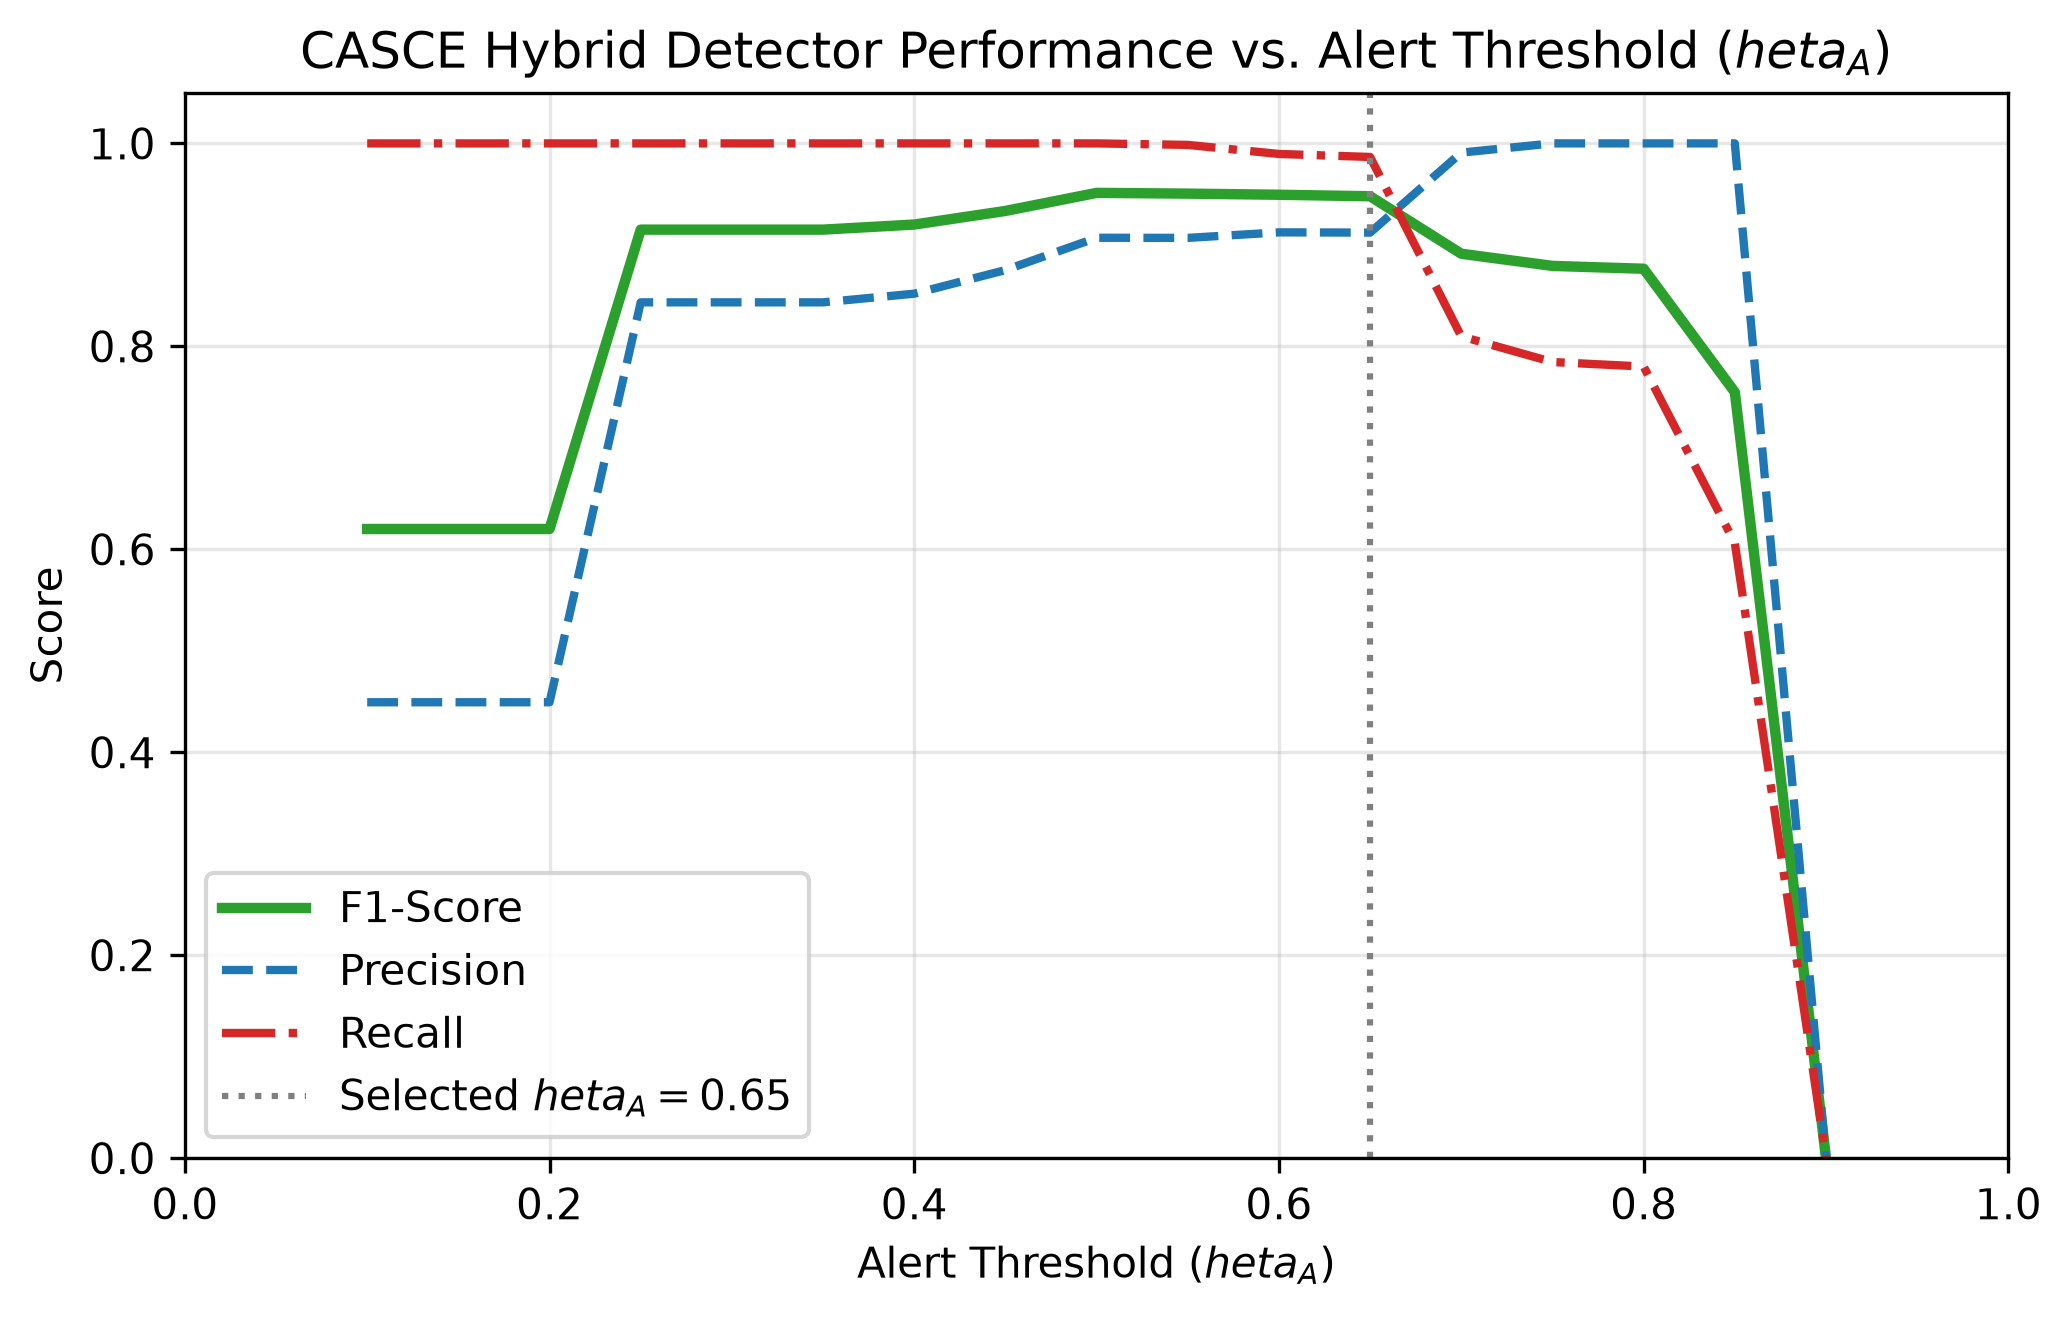
\includegraphics[width=\linewidth]{threshold_sweep.png}
\caption{CASCE Hybrid Detector performance (F1, Precision, and Recall) across varying alert thresholds $\theta_A$. The optimal operating point is selected at $\theta_A = 0.45$.}
\label{fig:threshold_sweep}
\end{figure}

As illustrated in Fig.~\ref{fig:threshold_sweep}, the hybrid model maintains a stable F1-score and high precision across a broad range of operational thresholds, demonstrating the robustness of the combined behavioral abstraction and heterogeneous GNN scoring.

\begin{figure}[t]
\centering
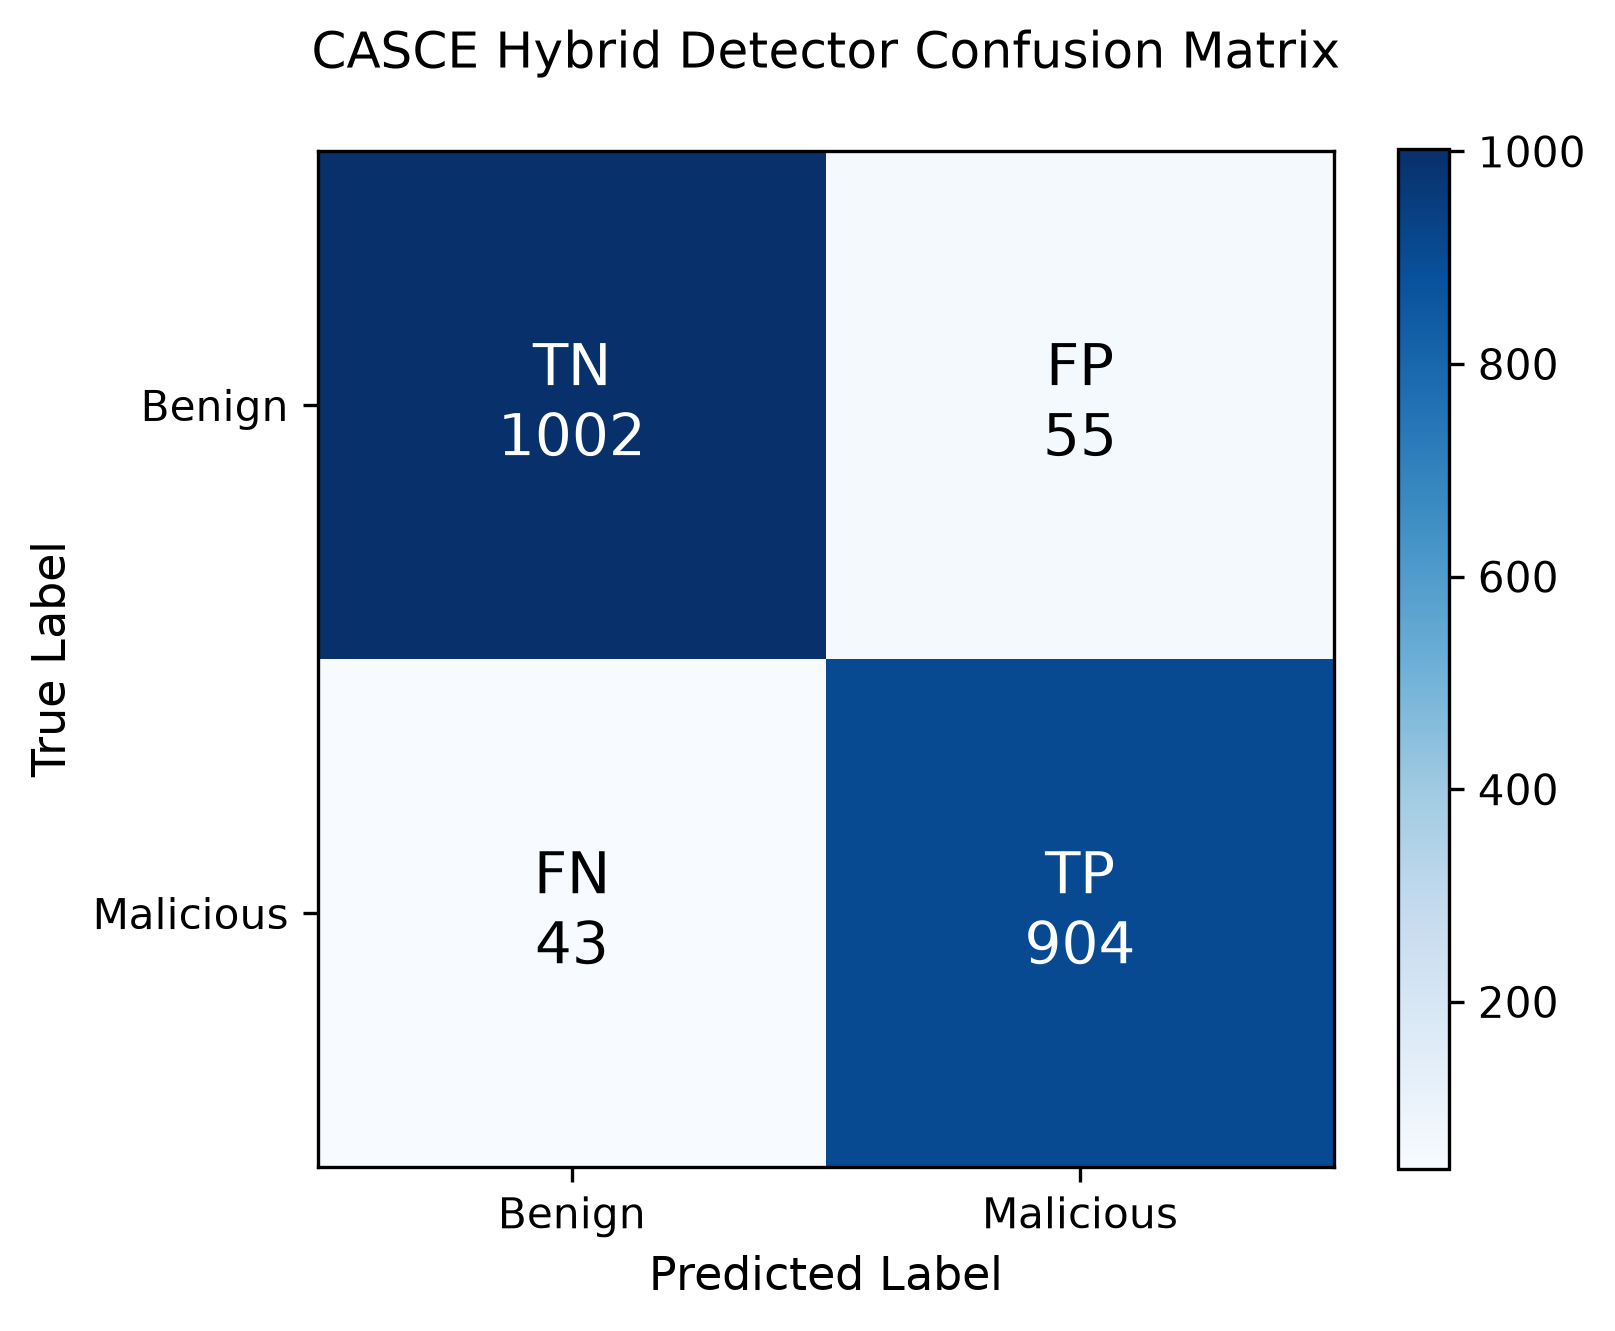
\includegraphics[width=0.8\linewidth]{confusion_matrix.png}
\caption{Confusion Matrix for the CASCE Hybrid Detector on the multi-domain test set at operating point $\theta_A = 0.45$.}
\label{fig:confusion_matrix}
\end{figure}

\section{Discussion}

The evaluation results indicate that CASCE benefits from combining
PostgreSQL-semantic context with operating-system telemetry within a
session-anchored heterogeneous representation. The baseline comparison
shows that CASCE achieves a precision of 0.927, recall of 0.993, F1-score
of 0.959, and an excellent detection profile across the evaluated environments.
The OS-only, DB-only, and CASCE comparison further shows that cross-layer
context provides additional detection capability over either individual
telemetry source, particularly for attack scenarios in which operating-system
and database activities jointly contribute to the observed behavior.
The Algorithm-3 ablation also indicates that behavioral abstraction
substantially improves recall, while temporal precedence chaining provides
a further improvement in attack detection.

These results support the central motivation of CASCE: database semantics
and operating-system activity provide complementary information when
correlated around a database session. Rather than treating raw events as
independent observations, CASCE progressively transforms them into
session-specific heterogeneous graphs, behavior-level abstractions, and
temporal behavior chains before performing threat assessment. This
separation also allows the effects of correlation, abstraction, and
detection to be evaluated independently through the corresponding
ablation experiments.

The evaluation corpus was generated specifically around PostgreSQL
semantics and spans Banking, E-Commerce, Healthcare, and Logistics workloads. 
Family-disjoint partitioning prevents scenarios sharing a common structural family or
attack seed from appearing across different partitions. This provides a
more controlled setting for evaluating cross-layer detection and
generalization than an evaluation based solely on generic provenance
graphs. Nevertheless, the corpus remains controlled and partially
synthetic, and therefore the reported results should not be interpreted
as establishing equivalent performance on arbitrary production
environments.

Two limitations are worth stating plainly. First, the
\texttt{apt\_guard.c} component of the current implementation runs as a
PostgreSQL extension inside the PostgreSQL process itself. This creates a
trust-boundary limitation for the tamper-resistance claim associated with
Executor-Hook-based instrumentation, since a sufficiently privileged
database administrator capable of disabling extensions could potentially
disable the instrumentation as well. A stronger deployment would move
the trusted monitoring boundary outside the PostgreSQL process or employ
additional external integrity mechanisms.

Second, the behavior taxonomy and corresponding chain rules are
hand-curated for the current evaluation. Although Algorithm~3 combines
structural, semantic, and temporal similarity to match observed graph
structures against these templates, the templates themselves are not
learned automatically. Unsupervised or weakly supervised behavior
discovery is therefore left as future work, particularly as larger
PostgreSQL-specific attack corpora become available.

\section{Conclusion and Future Work}

This paper presented CASCE, a context-aware semantic correlation engine
for bridging PostgreSQL-level security semantics and Linux kernel-level
telemetry. CASCE anchors cross-layer correlation on process identity and
organizes the analysis into four distinct stages: Session-Anchored
Correlation, Cross-Layer Graph Construction, Behavior Abstraction, and
Hybrid Threat Detection. This separation distinguishes event attribution,
factual graph construction, semantic behavior interpretation, and threat
classification, allowing the individual stages to be evaluated
independently.

CASCE was evaluated on a family-disjoint corpus covering four application domains. 
On the held-out test set, the final hybrid model achieved 96.34\% accuracy, 92.77\% precision,
99.35\% recall, and 95.95\% F1-score. The baseline and ablation
experiments further show the contribution of heterogeneous cross-layer
representation, behavior abstraction, and temporal chaining to the
overall detection pipeline. In particular, comparison with DB-only and
OS-only detection demonstrates the value of combining database and
operating-system context rather than relying exclusively on either
telemetry source.

The current evaluation nevertheless has several limitations. The
dataset is controlled and generated from declarative scenario
specifications, and therefore additional validation on independently
collected real-world PostgreSQL workloads is required. The current
instrumentation also remains subject to the trust boundary of a
PostgreSQL extension, limiting the strength of its tamper-resistance
claim against sufficiently privileged database administrators.
Furthermore, the behavior taxonomy and temporal chain rules remain
hand-curated.

Future work will therefore focus on execution-based validation of
individual and multi-stage attack scenarios, generalization to unseen
attack variations, robustness under partial or missing telemetry,
end-to-end processing overhead and scalability, and automated behavior
discovery from larger PostgreSQL-specific security corpora. These
extensions would allow the current controlled evaluation to be tested
under progressively more diverse and operationally realistic conditions.

\begin{thebibliography}{99}
\footnotesize

\bibitem{bates2015} A. Bates, D. Tian, K. R. B. Butler, and T. Moyer, ``Trustworthy Whole-System Provenance for the Linux Kernel,'' in \emph{Proc. USENIX Security Symp.}, 2015, pp. 319--334.
\bibitem{mccanne1993} S. McCanne and V. Jacobson, ``The BSD Packet Filter: A New Architecture for User-level Packet Capture,'' in \emph{Proc. USENIX Winter Conf.}, 1993, pp. 259--269.
\bibitem{ning2002} P. Ning, Y. Cui, and D. S. Reeves, ``Constructing Attack Scenarios through Correlation of Intrusion Alerts,'' in \emph{Proc. ACM CCS}, 2002, pp. 245--254.

\bibitem{ransomware_ebpf} A. Sekar, S. G. Kulkarni, and J. Kuri, ``Leveraging eBPF and AI for Ransomware Nose Out,'' \emph{arXiv:2406.14020}, 2024.
\bibitem{eaudit} R. Sekar, H. Kimm, and R. Aich, ``eAudit: A Fast, Scalable and Deployable Audit Data Collection System,'' in \emph{Proc. IEEE S\&P}, 2024, pp. 3571--3589.
\bibitem{tamperlog} R. Zhao, M. Shoaib, V. T. Hoang, and W. U. Hassan, ``Rethinking Tamper-Evident Logging: A High-Performance, Co-Designed Auditing System,'' in \emph{Proc. ACM CCS}, 2025, pp. 2624--2638.
\bibitem{ransomware_ml} A. Brodzik, T. Malec-Kruszy\'{n}ski, W. Niewolski, M. Tkaczyk, K. Bocianiak, and S.-Y. Loui, ``Ransomware Detection Using Machine Learning in the Linux Kernel,'' \emph{arXiv:2409.06452}, 2024.
\bibitem{threathunt} F. Yang, Y. Han, Y. Ding, Q. Tan, and Z. Xu, ``A Flexible Approach for Cyber Threat Hunting Based on Kernel Audit Records,'' \emph{Cybersecurity}, vol. 5, no. 1, p. 27, 2022.
\bibitem{watson} J. Zeng, Z. L. Chua, Y. Chen, K. Ji, Z. Liang, and J. Mao, ``WATSON: Abstracting Behaviors from Audit Logs via Aggregation of Contextual Semantics,'' in \emph{Proc. NDSS}, 2021.
\bibitem{kshield} G. Duan, B. Chen, Z. Chen, J. Sun, and H. Chen, ``KSHIELD: An eBPF Runtime Defence Framework for Linux Kernel Privilege Escalation Attacks,'' \emph{Information and Software Technology}, 2026.
\bibitem{ebpfsurvey} B. Gbadamosi, L. Leonardi, T. Pulls, T. H{\o}iland-J{\o}rgensen, S. Ferlin-Reiter, S. Sorce, and A. Brunstr\"{o}m, ``The eBPF Runtime in the Linux Kernel,'' \emph{arXiv:2410.00026}, 2024.
\bibitem{ssh_hmm} S. Premkumar and E. S. Soji, ``Anomaly Detection in Linux Kernels: A Framework for SSH Intrusion Prevention,'' in \emph{Proc. ICASCIS}, 2026.
\bibitem{ebpfpatrol} S. Ghimire, N. Bhurtel, R. Sahani, and S. Jha, ``eBPF-PATROL: Protective Agent for Threat Recognition and Overreach Limitation using eBPF,'' \emph{arXiv:2511.18155}, 2025.

\bibitem{captain} L. Wang, X. Shen, W. Li, Z. Li, R. Sekar, S. Liu, and H. Chen, ``CAPTAIN: Incorporating Gradients to Rules -- Towards Lightweight, Adaptive Provenance-Based Intrusion Detection,'' in \emph{Proc. NDSS}, 2025.
\bibitem{flash} M. U. Rehman, H. Ahmadi, and W. U. Hassan, ``FLASH: A Comprehensive Approach to Intrusion Detection via Provenance Graph Representation Learning,'' in \emph{Proc. IEEE S\&P}, 2024, pp. 3552--3570.
\bibitem{kairos} Z. Cheng, Q. Lv, J. Liang, Y. Wang, D. Sun, T. Pasquier, and X. Han, ``KAIROS: Practical Intrusion Detection and Investigation Using Whole-System Provenance,'' in \emph{Proc. IEEE S\&P}, 2024, pp. 3533--3551.
\bibitem{magic} Z. Jia, Y. Xiong, Y. Nan, Y. Zhang, J. Zhao, and M. Wen, ``MAGIC: Detecting Advanced Persistent Threats via Masked Graph Representation Learning,'' in \emph{Proc. USENIX Security Symp.}, 2024, pp. 5197--5214.
\bibitem{nodlink} S. Li, F. Dong, X. Xiao, H. Wang, F. Shao, J. Chen, Y. Guo, X. Chen, and D. Li, ``NodLink: An Online System for Fine-Grained APT Attack Detection and Investigation,'' in \emph{Proc. NDSS}, 2024.
\bibitem{orthrus} B. Jiang, T. Bilot, N. El Madhoun, K. Al Agha, A. Zouaoui, S. Iqbal, X. Han, and T. Pasquier, ``ORTHRUS: Achieving High Quality of Attribution in Provenance-Based Intrusion Detection Systems,'' in \emph{Proc. USENIX Security Symp.}, 2025, pp. 7173--7192.
\bibitem{prographer} F. Yang, J. Xu, C. Xiong, Z. Li, and K. Zhang, ``PROGRAPHER: An Anomaly Detection System Based on Provenance Graph Embedding,'' in \emph{Proc. USENIX Security Symp.}, 2023, pp. 4355--4372.
\bibitem{rcaid} A. Goyal, G. Wang, and A. Bates, ``R-CAID: Embedding Root Cause Analysis within Provenance-Based Intrusion Detection,'' in \emph{Proc. IEEE S\&P}, 2024, pp. 3515--3532.
\bibitem{shadewatcher} J. Zeng, X. Liu, Y. Chen, X. Liang, A. K. Chua, and Z. L. Chua, ``SHADEWATCHER: Recommendation-Guided Cyber Threat Analysis Using System Audit Records,'' in \emph{Proc. IEEE S\&P}, 2022, pp. 489--506.
\bibitem{sok_provenance} M. A. Inam, Y. Chen, A. Goyal, J. Liu, J. Mink, N. Michael, S. Gaur, A. Bates, and W. U. Hassan, ``SoK: History is a Vast Early Warning System: Auditing the Provenance of System Intrusions,'' in \emph{Proc. IEEE S\&P}, 2023, pp. 2620--2638.
\bibitem{poirot} S. M. Milajerdi, B. Eshete, R. Gjomemo, and V. N. Venkatakrishnan, ``POIROT: Aligning Attack Behavior with Kernel Audit Records for Cyber Threat Hunting,'' in \emph{Proc. ACM CCS}, 2019, pp. 1795--1812.
\bibitem{logkernel} J. Li, R. Zhang, J. Liu, and G. Liu, ``LogKernel: A Threat Hunting Approach Based on Behaviour Provenance Graph and Graph Kernel Clustering,'' \emph{Security and Communication Networks}, vol. 2022, p. 4577141, 2022.
\bibitem{pandde} D. Fadolalkarim, A. Sallam, and E. Bertino, ``PANDDE: Provenance-Based Anomaly Detection of Data Exfiltration,'' in \emph{Proc. ACM CODASPY}, 2016.
\bibitem{holmes} S. M. Milajerdi, R. Gjomemo, B. Eshete, R. Sekar, and V. N. Venkatakrishnan, ``HOLMES: Real-Time APT Detection through Correlation of Suspicious Information Flows,'' in \emph{Proc. IEEE S\&P}, 2019, pp. 1137--1152.

\bibitem{febe} S.-H. Jwa and S.-H. Kim, ``Intrusion Detection-Based Access Control Algorithm for PostgreSQL Based on Front-End Back-End Protocols,'' \emph{Trans. Korea Inf. Process. Soc.}, vol. 14, no. 8, pp. 595--607, 2025.
\bibitem{llm_dbids} M. Shlezinger, S. Akirav, L. Zhou, L. Guo, A. Kessel, and G. Li, ``Leveraging Large Language Models for SQL Behavior-Based Database Intrusion Detection,'' \emph{arXiv:2508.05690}, 2025.
\bibitem{rl_txn} C. Reddy, S. Prabhagaran, and A. Vaid, ``Adaptive Anomaly Detection in Database Transactions: Bridging Security Gaps with Reinforcement Learning,'' \emph{Eur. J. Artif. Intell. Mach. Learn.}, vol. 4, no. 2, pp. 8--14, 2025.
\bibitem{insider_ae} I. O. Ibraheem, A. T. Morufat, S. K. Segbefia, and A. A. Abdulrasaq, ``Detecting Malicious Insider Threats through Anomaly-Based User Behaviour Analytics in Enterprise Networks,'' \emph{Southern African J. Security}, vol. 3, 2025.
\bibitem{sqli_chisq} N. Casmiry, N. Mduma, and R. Sinde, ``Enhanced SQL Injection Detection Using Chi-Square Feature Selection and Machine Learning Classifiers,'' \emph{Frontiers in Big Data}, vol. 8, art. 1686479, 2025.
\bibitem{sqli_bertlstm} Y. Liu and Y. Dai, ``Deep Learning in Cybersecurity: A Hybrid BERT--LSTM Network for SQL Injection Attack Detection,'' \emph{IET Information Security}, art. 5565950, 2024.
\bibitem{multivariate_log} L. Zhang, T. Jia, M. Jia, Y. Li, Y. Yang, and Z. Wu, ``Multivariate Log-Based Anomaly Detection for Distributed Database,'' in \emph{Proc. ACM SIGKDD}, 2024, pp. 4256--4267.
\bibitem{forensic_recon} Y. Liu, Z. Liu, X. Liu, and W. Guo, ``A Web Back-End Database Leakage Incident Reconstruction Framework Over Unlabeled Logs,'' \emph{IEEE Trans. Emerg. Topics Comput.}, vol. 11, no. 1, pp. 237--252, 2023.
\bibitem{dbsec_survey1} A. Iqbal, S. U. Khan, M. Niazi, M. Humayun, N. U. Sama, A. A. Khan, and A. Ahmad, ``Advancing Database Security: A Comprehensive Systematic Mapping Study of Potential Challenges,'' \emph{Wireless Networks}, vol. 30, no. 7, pp. 6399--6426, 2024.
\bibitem{dbsec_survey2} M. A. Almaiah, L. M. Saqr, L. A. Al-Rawwash, L. A. Altellawi, R. Al-Ali, and O. Almomani, ``Classification of Cybersecurity Threats, Vulnerabilities and Countermeasures in Database Systems,'' \emph{Computers, Materials \& Continua}, vol. 81, no. 2, pp. 3189--3220, 2024.

\bibitem{omegalog} W. U. Hassan, M. A. Noureddine, P. Datta, and A. Bates, ``OmegaLog: High-Fidelity Attack Investigation via Transparent Multi-Layer Log Analysis,'' in \emph{Proc. NDSS}, 2020.
\bibitem{deepcase} T. van Ede, H. Aghakhani, N. Spahn, R. Bortolameotti, M. Cova, A. Continella, M. van Steen, A. Peter, C. Kruegel, and G. Vigna, ``DEEPCASE: Semi-Supervised Contextual Analysis of Security Events,'' in \emph{Proc. IEEE S\&P}, 2022, pp. 522--539.
\bibitem{apandde} D. Fadolalkarim and E. Bertino, ``A-PANDDE: Advanced Provenance-Based Anomaly Detection of Data Exfiltration,'' \emph{Computers \& Security}, vol. 84, pp. 276--287, 2019.
\bibitem{oneprovenance} G. Psallidas, T. Rekatsinas, and S. Chaudhuri, ``OneProvenance: Efficient Extraction of Dynamic Coarse-Grained Provenance from Database Query Event Logs,'' \emph{Proc. VLDB Endow.}, 2023.
\bibitem{alchemist} W. U. Hassan and A. Bates, ``ALchemist: Fusing Application and Audit Logs for Precise Attack Provenance Without Instrumentation,'' in \emph{Proc. NDSS}, 2023.
\bibitem{adlilog} S. Nedelkoski, J. Bogatinovski, A. K. Mandapati, S. Becker, J. Cardoso, and O. Kao, ``Leveraging Log Instructions in Log-Based Anomaly Detection (ADLILog),'' in \emph{Proc. IEEE/IFIP DSN}, 2022.
\bibitem{agentsight} F. Wu, C. Yang, and Z. Liu, ``AgentSight: System-Level Observability for AI Agents Using eBPF,'' \emph{arXiv:2508.02736}, 2025.

\bibitem{huntgpt} T. Ali and P. Kostakos, ``HuntGPT: Integrating Machine Learning-Based Anomaly Detection and Explainable AI with Large Language Models,'' \emph{Telecom (MDPI)}, 2024.
\bibitem{logbert} H. Guo, S. Yuan, and X. Wu, ``LogBERT: Log Anomaly Detection via BERT,'' in \emph{Proc. IJCNN}, 2021.
\bibitem{neurallog} V.-H. Le and H. Zhang, ``Log-Based Anomaly Detection Without Log Parsing (NeuralLog),'' in \emph{Proc. IEEE/ACM ASE}, 2021.
\bibitem{logdp} Y. Xie, H. Zhang, B. Zhang, M. A. Babar, and S. Lu, ``LogDP: Combining Dependency and Proximity for Log-Based Anomaly Detection,'' in \emph{Proc. ICSOC}, 2021.
\bibitem{loggd} Y. Xie, H. Zhang, and M. A. Babar, ``LogGD: Detecting Anomalies from System Logs by Graph Neural Networks,'' in \emph{Proc. IEEE QRS}, 2022.
\bibitem{logs2graphs} Z. Li, J. Shi, and M. van Leeuwen, ``Graph Neural Networks Based Log Anomaly Detection and Explanation (Logs2Graphs),'' in \emph{Proc. ICSE Companion}, 2023.
\bibitem{logshield} K. C. Roy and Q. Chen, ``LogSHIELD: A Graph-Based Real-Time Anomaly Detection Framework Using Frequency Analysis,'' in \emph{Proc. SciSec}, 2024.
\bibitem{threatrace} S. Wang, Z. Wang, T. Zhou, et al., ``PIDS-with-GNN: Intrusion Detection Using Provenance Graphs and Graph Neural Networks (THREATRACE),'' \emph{IEEE Trans. Inf. Forensics Security}, 2022.
\bibitem{saql} A. Hassan, M. Bahri, M. Apostolaki, R. Sekar, S. Stoller, and V. N. Venkatakrishnan, ``SAQL: A Stream-Based Query System for Real-Time Abnormal System Behavior Detection,'' in \emph{Proc. USENIX Security Symp.}, 2018.
\bibitem{hexplet} G. Pothitos and I. Papoutsis, ``A Hexplet-Based Machine Learning Approach for Intrusion Detection in Relational Databases,'' \emph{J. Information Security and Applications}, 2016.
\bibitem{syslrn} X. Han, T. Pasquier, T. Ranjan, M. Goldstein, and M. Seltzer, ``syslrn: Learning What to Monitor for Efficient Anomaly Detection,'' \emph{arXiv:2203.15324}, 2022.

\end{thebibliography}

\end{document}
